%-----------------------------------------------------------Header Starts--------------------------------------

\documentclass[main.tex]{subfiles}

%-----------------------------------------------------------Header Ends--------------------------------------


\graphicspath{ {./image_literature/} }



\begin{document}

\chapter{Literature Review}

\thispagestyle{empty}

\pagestyle{fancy}
\fancyhf{}

\rhead{Page \thepage}
\lhead{\chaptername \ \thechapter}

The requirement of dilute magnetic semiconductor is its non-volatile ferromagnetism which must have non-zero spin polarization at fermi level. To this day, extensive research have been performed on dilute magnetic semiconductors. During exploitation the prospects of DMS in any material a number of questions must be carefully resolved. The primary questions are definitely about the structural purity of the sample such as any presence of 2nd phase in X-ray and electron diffraction study, any presence of metallic cluster of dopants in X-ray photoelectron study, any presence of satellite peaks due to oxygen vacancies in the valence band spectra etc. If these questions are resolved then next questions will come forward which are about the spin polarization nature. Before going further on the spin polarization in DMS, it is required to revisit the concepts of three fascinating photoemission spectroscopy techniques which are X-ray absorption spectroscopy (XAS), X-ray magnetic circular dichroism (XMCD) and angle resolved X-ray photoelectron spectroscopy (ARPES). This chapter begins with a plain explanation of these powerful spectroscopy techniques. 

\section{\capitalisewords{X-ray absorption spectroscopy}}

X-ray absorption spectroscopy provides a clear picture of valence shell by exciting a core level electron to an empty valence shell. In magnetic materials, the valence shell is typically 3d or 4f and they are partially filled. The excited photoelectrons take position in the empty places in d or f orbitals and eventually return to ground state by emitting a fluroscent/auger electrons. The detector in XAS capture and analyze the auger electrons. Peaks are splitted due to spin-orbit interaction of core level electrons. 

\begin{figure}[!htb]
\centering
	\begin{subfigure}[h]{0.4\textwidth}
		\centering
		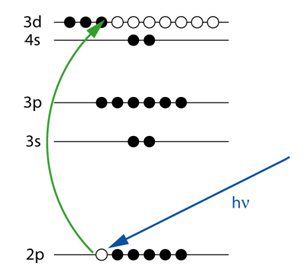
\includegraphics[width=\linewidth]{XAS1}
  		\caption{Excitation of a core level electron to valence shell}
   		%\label{fig:sub-first}
	\end{subfigure}
	\begin{subfigure}[h]{0.51\textwidth}
  		\centering
  		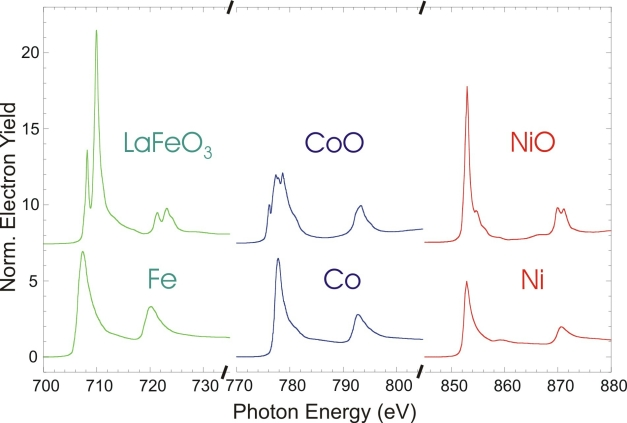
\includegraphics[width=\linewidth]{XAS3}
  		\caption{Difference of X-ray absorption in metal and oxide}
  		%\label{fig:sub-second}
	\end{subfigure}
\caption{Schematic principle of X-ray absorption spectroscopy. (images are taken from the webpage of SLAC, Stanford University)}
\label{fig:fig}

\end{figure}
\FloatBarrier

Usually metal shows 2 peaks in XAS while oxides show multiplets as spin-orbit interactions are more localized in oxide materials. Total intensity of the peaks is proportional to the empty d or f orbital density of states. Although XAS can depict the density of states in valence band but it cannot provide any details of spin polarization. For example, the electron configuration of Fe is [Ar] $3d^{6}$ $4s^{2}$ and for $Fe^{3+}$ it is [Ar] $3d^{5}$. 

\begin{figure}[!htb]
\centering
	\begin{subfigure}[h]{0.5\textwidth}
		\centering
		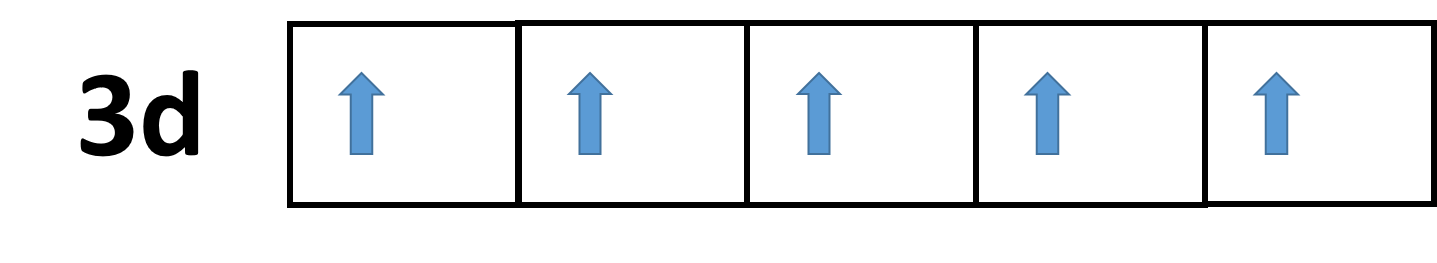
\includegraphics[width=\linewidth]{fe_3d_1}
  		\caption{3d orbital in ground state}
   		%\label{fig:sub-first}
	\end{subfigure}
	\begin{subfigure}[h]{0.5\textwidth}
  		\centering
  		
\includegraphics[width=\linewidth]{fe_3d_2}
  		\caption{crystal field splitting of 3d orbital}
  		%\label{fig:sub-second}
	\end{subfigure}
\caption{Difference in 3d orbital due to crystal field splitting in $Fe^{3+}$}
\label{fig:fig}

\end{figure}
\FloatBarrier

In XAS, the photo-excited core level electrons just fill up the empty states in 3d orbital and there will be no difference in the observed absorption spectra for crystal field splitting. During investigation of spin polarization, observation of only density of states is not enough. For example, XAS cannot differentiate between the density of states for 5 spin-up electrons showed in Fig 2.2(a) and the density of states for 3 spin-up $\&$ 2 spin-down electrons showed in Fig 2.2(b). This problem has been resolved by X-ray magnetic circular dichroism spectroscopy. 

\section{\capitalisewords{X-ray magnetic circular dichroism}}

X-ray magnetic circular dichroism (XMCD) is a special feature of X-ray absorption spectroscopy (XAS). Dichroism means polarization dependent light absorption of any materials. In simple terms, XMCD is basically an XAS placed in a magnetic field where the incident light is polarized. The left or right circularly polarized photons transfer their angular momentum to the core level electrons. Since change of spin momentum is forbidden in electric dipole transition, the photo-ejected electrons carry the same angular momentum to the valence band. The theory of XMCD was first proposed by Erskine \textit{et al.} in 1986 and the experimental proof of XMCD was demonstrated by Gerrit van der Laan \textit{et al.} in 1986 \cite{erskine1975calculation, van1986experimental}. A list of synchroton facilities for XMCD around the world is given in the reference \cite{wilhelm2013magnetic}. \\

Fig 2.3 shows a schematic mechanism of XMCD. At ground state, 2p electrons of Cobalt metal are usually splitted in \(j=\frac{3}{2}\) level ($L_3$ edge) and \(j=\frac{1}{2}\) level ($L_2$ edge). It is noteworthy to mention that spin and orbit are coupled parallel in $L_3$ edge and antiparallel in $L_2$ edge. At first, the right circularly polarized incident light excites the 2p electrons which are parallel to the helicity of the light (spin-up electrons). Similarly the left circularly polarized light excites the antiparallel electrons at 2p core states (spin-down electrons). These electrons carry the angular momentum and fill up the unoccupied empty states in 3d orbital. The net difference of available places for spin-up and spin-down electrons in unoccupied 3d orbitals can be understood by the XMCD graph. 

\begin{figure}[!htb]
	\centering
	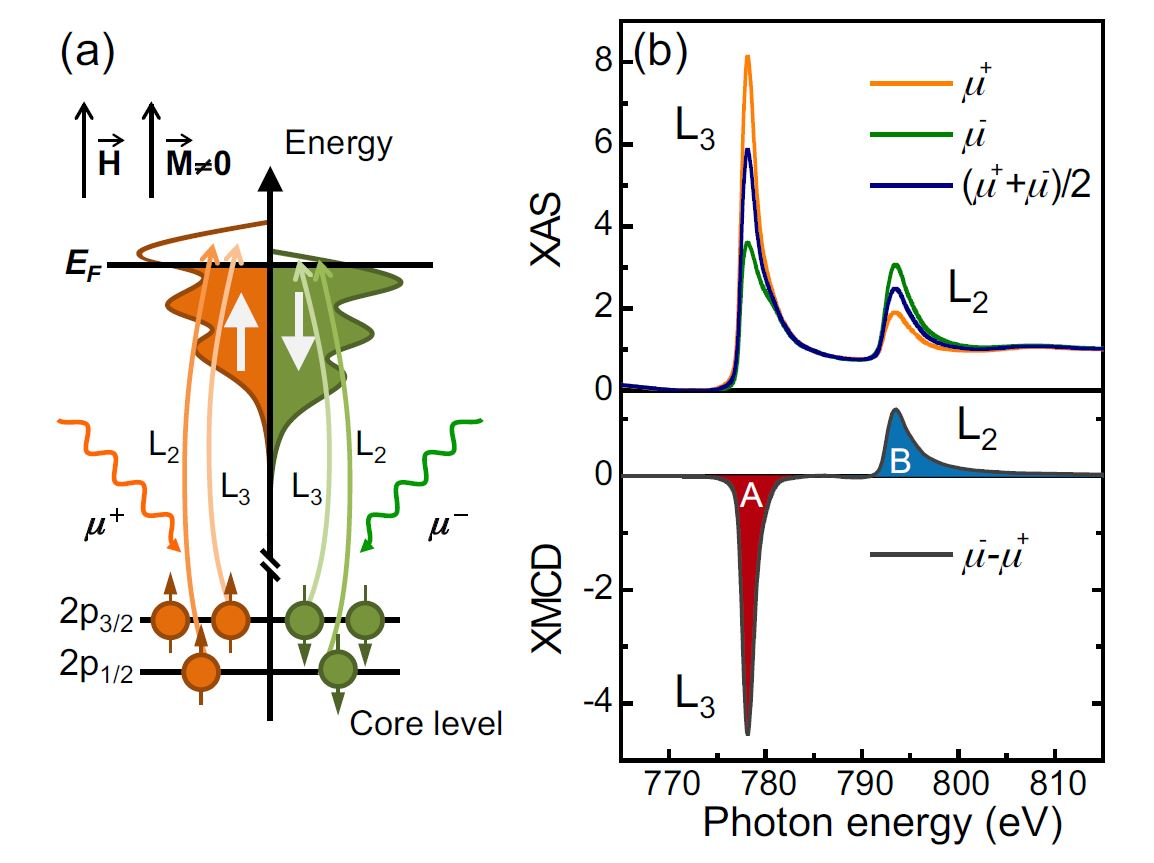
\includegraphics[width=0.85\linewidth]{xmcd}
	\caption{(a)Schematic principle of X-ray magnetic circular dichroism (XMCD) (b) Difference between XAS and XMCD principle \cite{van2014x}}
	\label{fig:TEM_PT}
\end{figure}
\FloatBarrier

\section{\capitalisewords{Angle resolved photoemission spectroscopy}}

Angle resolved photo emission spectroscopy is the characterization technique for direct observation of the electronic band structure of any crystalline material. 

\begin{figure}[!htb]
\centering
	\begin{subfigure}[h]{0.5\textwidth}
		\centering
		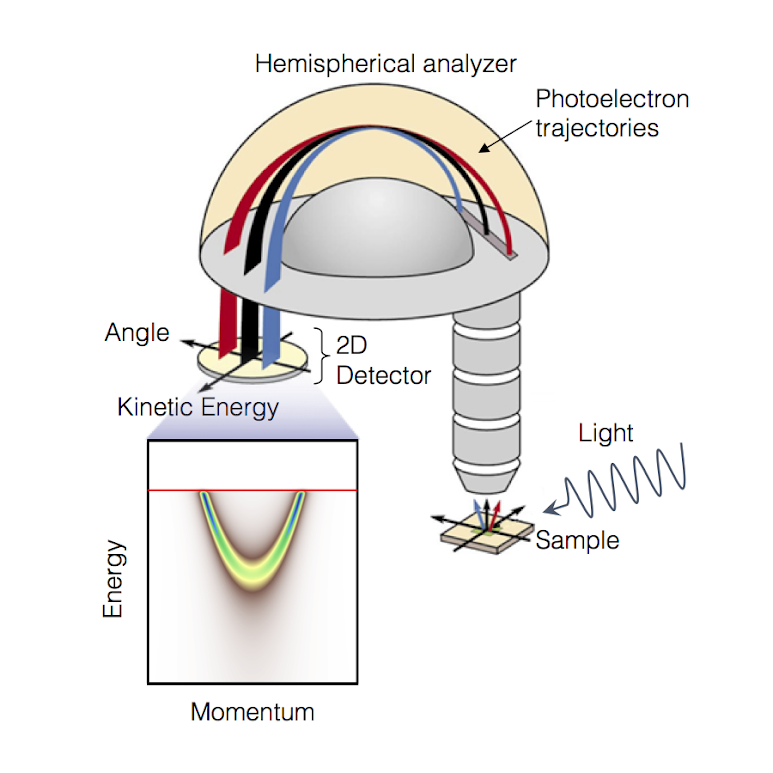
\includegraphics[width=\linewidth]{arpes1}
  		\caption{}
   		%\label{fig:sub-first}
	\end{subfigure}
	\begin{subfigure}[h]{0.48\textwidth}
  		\centering
  		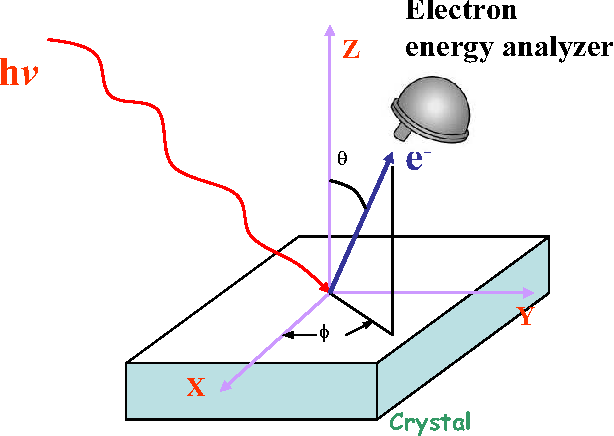
\includegraphics[width=\linewidth]{arpes2}
  		\caption{}
  		%\label{fig:sub-second}
	\end{subfigure}
\caption{Schematic diagram of angle resolved photoemission spectroscopy}
\label{fig:fig}

\end{figure}
\FloatBarrier

Like the other photoemission spectroscopy, ARPES is based on the photoelectric effect which was pioneered by Einstein. When a sample is irradiated by incident light with sufficient energy, an electron from the surface of the material can absorb the energy of photon and escape the surface. The kinetic energy required for this process is \(h\nu-\phi\) ($h\nu$ is the photon energy and $\phi$ is the work function of the material). ARPES measures the kinetic energy of a photoelectron and calculates its original binding energy using the energy conservation law. Electrons having different momentum will escape from the surface at different angles and hence the momentum resolution of the photoejected electrons can be determined by analyzing the angle of the photoemission. 

\section{Recent advances in DMS research}

This section will briefly present a review on recent progress in DMS research. Over last few decades extensive research were performed on DMS properties in III-V, II-VI and oxide materials. The seminal research work by Munekata \textit{et al.} first demonstrated the DMS properties in III-V materials \cite{munekata1989diluted}. In their work, they have grown $In_{(1-x)}Mn_{x}As$ (x $\leq 0.18$) on both InAs and GaAs substrates by molecular beam epitaxy. The films showed intrinsic semiconducting behavior (n-type) but the curie temperature was far below room temperature. Hayashi \textit{et al.} found extraordinary magnetoresistance in $Ga_{(1-x)}Mn_{x}As$ \cite{hayashi1997magnetic}. The curie temperature and magnetization were increased with Mn concentration. Matsukura \textit{et al.} explained that the ferromagnetism observed in $Ga_{(1-x)}Mn_{x}As$ follows Ruderman-Kittel-Kasuya-Yosida (RKKY) exchange interaction \cite{matsukura1998transport}.

\begin{figure}[!htb]
\centering
	\begin{subfigure}[h]{0.5\textwidth}
		\centering
		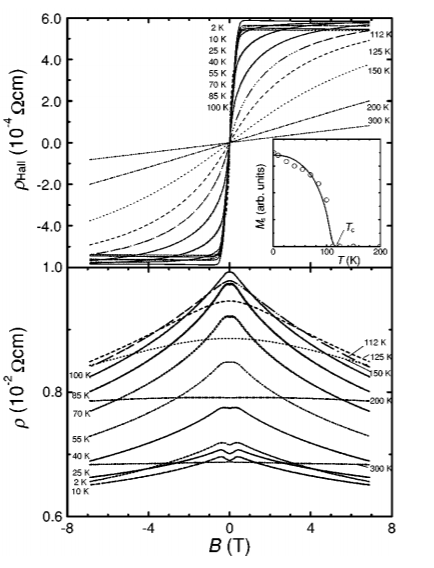
\includegraphics[width=\linewidth]{matsukura}
  		\caption{}
   		%\label{fig:sub-first}
	\end{subfigure}
	\begin{subfigure}[h]{0.46\textwidth}
  		\centering
  		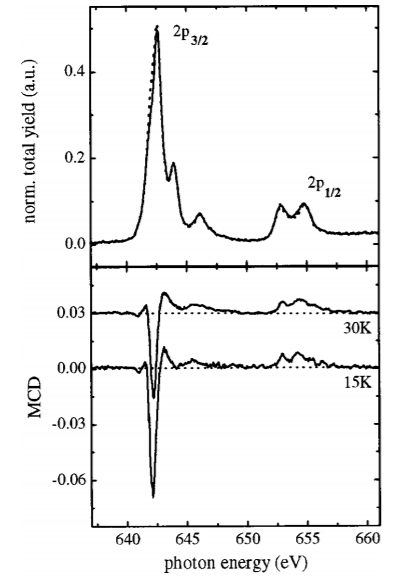
\includegraphics[width=\linewidth]{ohldag}
  		\caption{}
  		%\label{fig:sub-second}
	\end{subfigure}
\caption{(a) Magnetic-field vs. Hall resistivity $\rho_{Hall}$ and resistivity $\rho$ of $Ga_{(1-x)}Mn_{x}As$ vs. temperature. Mn concentration is x=0.053. The change of spontaneous magnetization $M_{s}$ with temperature is showed in inset \cite{matsukura1998transport} (b) X-ray absorption and X-ray magnetic circular dichroism spectra of $Ga_{0.98}Mn_{0.02}As$ \cite{ohldag2000magnetic}} 
\label{fig:fig}

\end{figure}
\FloatBarrier

Khalid \textit{et al.} found strong spin polarization at fermi level in $In_{0.95}Mn_{0.05}P$ sample which showed intrinsic semiconducting behavior and negative magnetoresistance \cite{khalid2014ferromagnetism}. Scarpulla \textit{et al.} reported carrier mediated ferromagnetism in $Ga_{0.94}Mn_{0.06}P$ where strongly localized hole states are created just above the valence band due to Mn doping \cite{scarpulla2005ferromagnetism}. But for both $Ga_{(1-x)}Mn_{x}P$ and $In_{(1-x)}Mn_{x}P$ the curie temperature remains around 60 K. 

\begin{figure}[!htb]
\centering
	\begin{subfigure}[h]{0.45\textwidth}
		\centering
		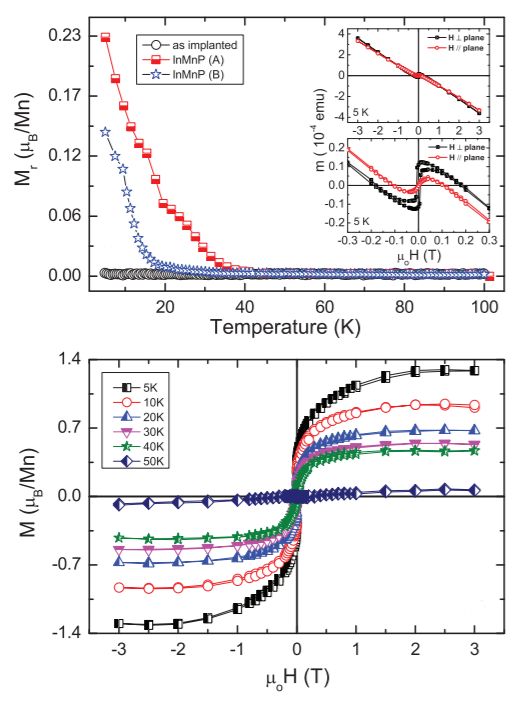
\includegraphics[width=\linewidth]{khalid1}
  		\caption{}
   		%\label{fig:sub-first}
	\end{subfigure}
	\begin{subfigure}[h]{0.47\textwidth}
  		\centering
  		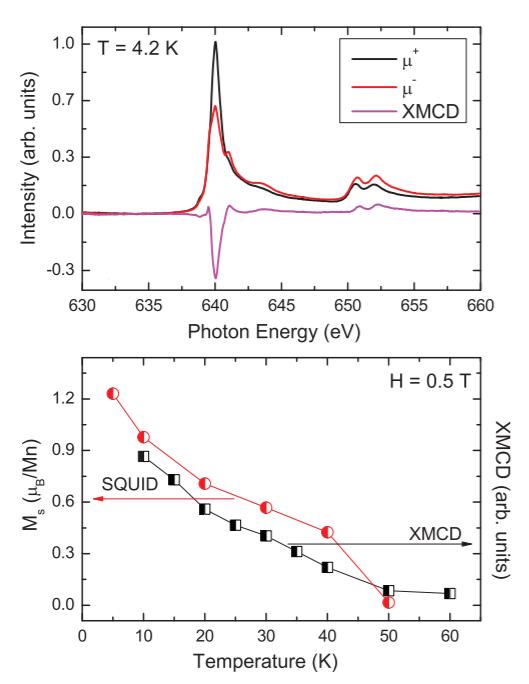
\includegraphics[width=\linewidth]{khalid2}
  		\caption{}
  		%\label{fig:sub-second}
	\end{subfigure}
\caption{(a) Magnetization vs. temperature of as-implanted and laser annealed (A and B) $In_{0.95}Mn_{0.05}P$ samples (b) XAS and XMCD study of $In_{0.95}Mn_{0.05}P$ \cite{khalid2014ferromagnetism}} 
\label{fig:fig}

\end{figure}
\FloatBarrier

Gray \textit{et al.} experimentally proved the half-metallic behavior of $Ga_{0.97}Mn_{0.03}As$ by analyzing the electronic band structure using Hard X-ray angle resolved photoemission spectroscopy \cite{gray2012bulk}. The Mn induced density of states were observed between fermi level and valence band maxima in their experiment.

\begin{figure}[!htb]
	\centering
	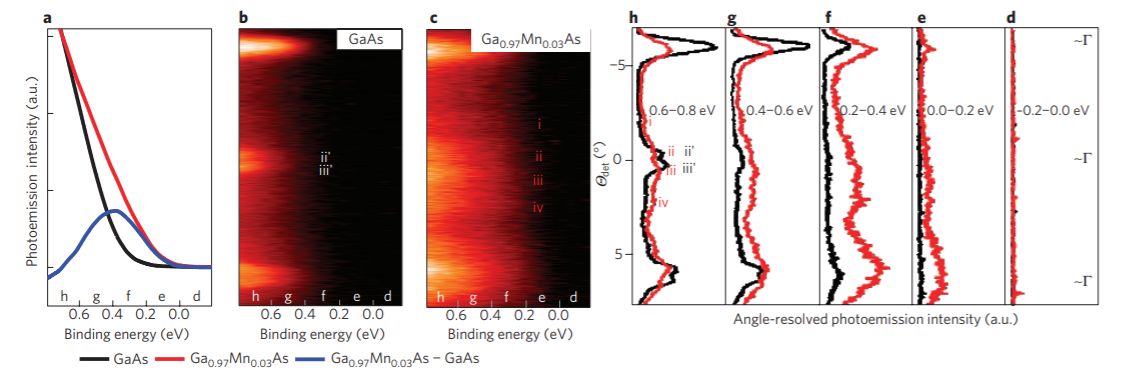
\includegraphics[width=0.99\linewidth]{gray}
	\caption{Experimental observation of half-metallic behavior in $Ga_{0.97}Mn_{0.03}As$ by Hard X-ray angle resolved photoemission spectroscopy \cite{gray2012bulk}}
	\label{fig:TEM_PT}
\end{figure}
\FloatBarrier

 Kobayashi \textit{et al.} also reported half-metallic behavior of $Ga_{0.975}Mn_{0.025}As$ in their seminal research paper \cite{kobayashi2014unveiling}. Nemvsak \textit{et al.} also reported half-metallic behavior in $Ga_{0.95}Mn_{0.05}As$ by using standing wave angle resolve photoemission spectroscopy (SW-ARPES) \cite{nemvsak2018element}. Keqi \textit{et al.} investigated the electronic structure of $Ga_{0.98}Mn_{0.02}P$ by using hard X-ray angle resolved photoemission spectroscopy and observed Mn induced impurity states near valence band maxima \cite{keqi2018electronic}.

\begin{figure}[!htb]
	\centering
	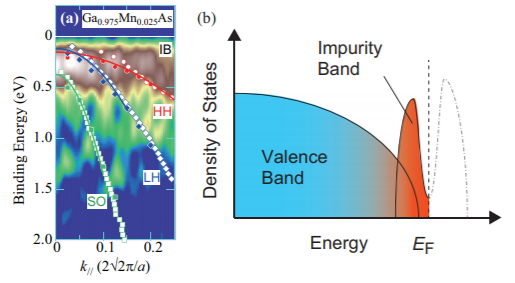
\includegraphics[width=0.8\linewidth]{kobayashi}
	\caption{Experimental observation of half-metallic behavior in $Ga_{0.975}Mn_{0.025}As$ by soft X-ray angle resolved photoemission spectroscopy \cite{kobayashi2014unveiling}}
	\label{fig:TEM_PT}
\end{figure}
\FloatBarrier

\begin{figure}[!htb]
	\centering
	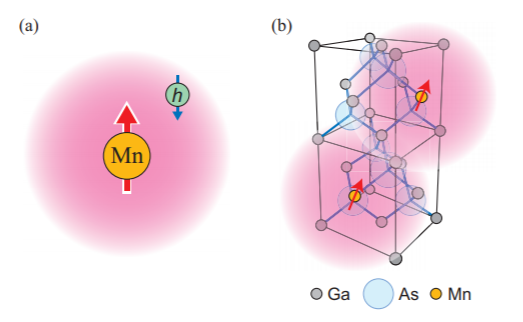
\includegraphics[width=0.8\linewidth]{kobayashi2}
	\caption{(a) Bound magnetic polaron controlling the ferromagnetism in $Ga_{0.975}Mn_{0.025}As$. (b) Schematic image of magnetic interaction in $Ga_{0.975}Mn_{0.025}As$ crystal structure \cite{kobayashi2014unveiling}}
	\label{fig:TEM_PT}
\end{figure}
\FloatBarrier

Furdyna \textit{et al.} first reported II-VI based dilute magnetic semiconductors ($Cd_{(1-x)}Mn_{x}Se$ and $Hg_{(1-x)}Mn_{x}Te$) in 1988 \cite{furdyna1988diluted}. Zhao \textit{et al.} reported short-range magnetic ordering in $Zn_{(1-x)}Cr_{x}Te$ \cite{zhao2006chemical}. Observation of similar short-range ferromagnetic interaction in II-VI based DMS have been reported in many literatures in last few decades \cite{haury1997observation, yang2010origin, dietl2010ten}. 

\begin{figure}[!htb]
	\centering
	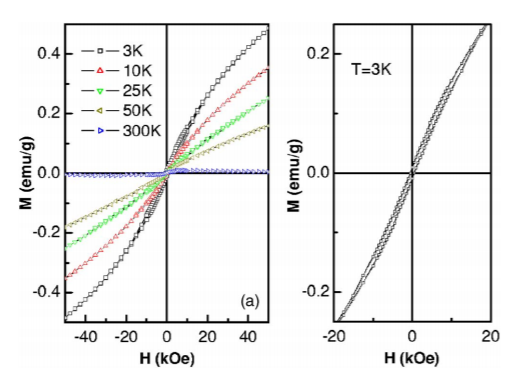
\includegraphics[width=0.8\linewidth]{zhao}
	\caption{Magnetization vs. applied field in $Zn_{(1-x)}Cr_{x}Te$ \cite{zhao2006chemical}}
	\label{fig:TEM_PT}
\end{figure}
\FloatBarrier

Matsumoto \textit{et al.} first demonstrated the intrinsic ferromagnetism in Co:Ti$O_2$ which showed high curie temperature \cite{matsumoto2001room}. This groundbreaking discovery led to extensive research on DMS in oxide based materials since 2001 \cite{coey2005donor, philip2006carrier, coey2005high, dietl2008origin, coey2008oxide}. Yamada \textit{et al.} reported electrically induced ferromagnetism in $Ti_{0.90}Co_{0.10}O_{2}$ at room temperature \cite{yamada2011electrically}. Saadaoui \textit{et al.} reported intrinsic ferromagnetism observed in $Ti_{0.95}Co_{0.05}O_{2}$ thin film is controlled by oxygen vacancy \cite{saadaoui2016intrinsic}. Several seminal research works also exhibit intrinsic carrier mediated ferromagnetism in other non-magnetic oxides like ZnO, $In_{2}O_{3}$, Ce$O_2$ \cite{yi2010ferromagnetism, sun2008evidence, krishna2015structural, pellicer2013mesoporous, farvid2013influence, gao2007ferromagnetic, thurber2007ferromagnetism, paidi2019role}.

\begin{figure}[!htb]
\centering
	\begin{subfigure}[h]{0.45\textwidth}
		\centering
		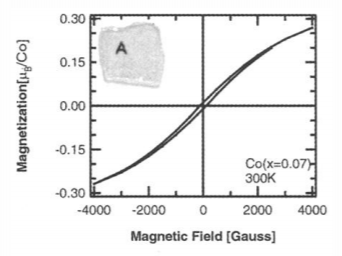
\includegraphics[width=\linewidth]{matsumo1}
  		\caption{}
   		%\label{fig:sub-first}
	\end{subfigure}
	\begin{subfigure}[h]{0.47\textwidth}
  		\centering
  		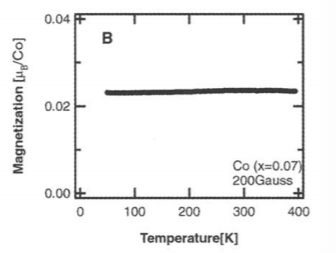
\includegraphics[width=\linewidth]{matsumo2}
  		\caption{}
  		%\label{fig:sub-second}
	\end{subfigure}
\caption{(a) Magnetization vs. applied field (b) Magnetization vs. temperature graph of $Ti_{0.93}Co_{0.07}O_{2}$ sample \cite{matsumoto2001room}} 
\label{fig:fig}

\end{figure}
\FloatBarrier

\begin{figure}[!htb]
\centering
	\begin{subfigure}[h]{0.42\textwidth}
		\centering
		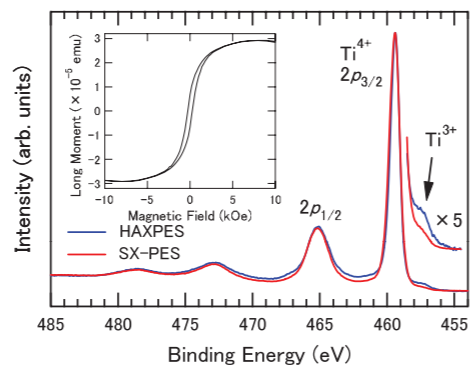
\includegraphics[width=\linewidth]{ohtsuki}
  		\caption{Soft X-ray and Hard X-ray photoemission spectroscopy of $Ti_{0.95}Co_{0.05}O_{2}$ thin film \cite{ohtsuki2011role}}
   		%\label{fig:sub-first}
	\end{subfigure}
	\begin{subfigure}[h]{0.5\textwidth}
  		\centering
  		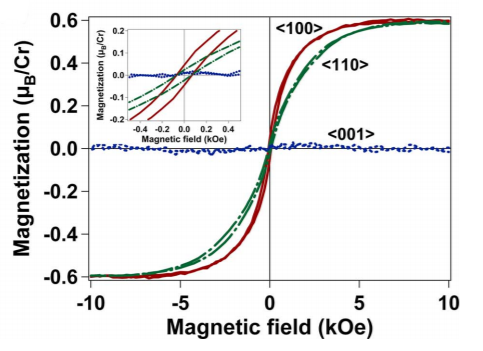
\includegraphics[width=\linewidth]{kaspar}
  		\caption{Magnetization vs. applied field in $Ti_{0.91}Co_{0.09}O_{2}$ thin film \cite{kaspar2006ferromagnetism}}
  		%\label{fig:sub-second}
	\end{subfigure}
\caption{Intrinsic ferromagnetism in transition metal doped $TiO_{2}$ thin films} 
\label{fig:fig}

\end{figure}
\FloatBarrier

\begin{figure}[!htb]
	\centering
	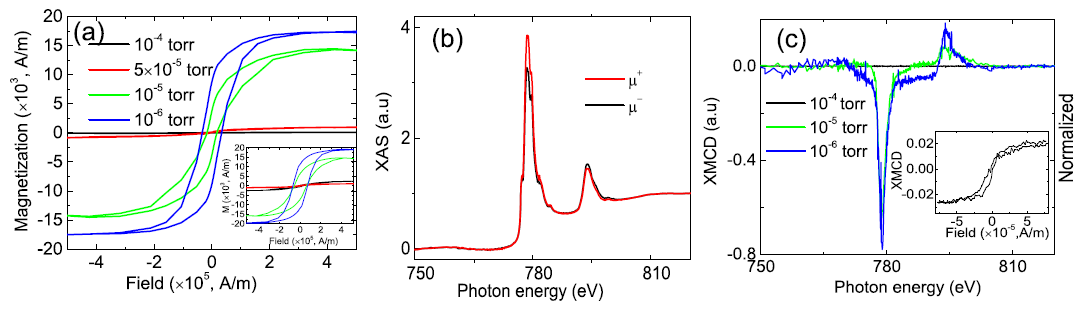
\includegraphics[width=0.99\linewidth]{saadaoui}
	\caption{(a) Magnetization vs. applied field (b) XAS and (c) XMCD spectra of $Ti_{0.95}Co_{0.05}O_{2}$ thin film \cite{saadaoui2016intrinsic}}
	\label{fig:TEM_PT}
\end{figure}
\FloatBarrier

\begin{figure}[!htb]
	\centering
	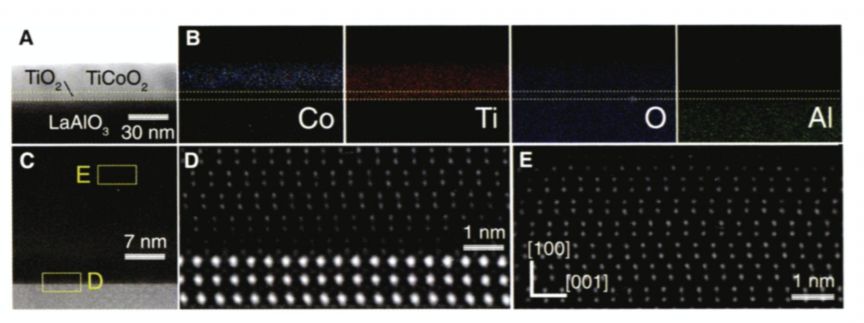
\includegraphics[width=0.99\linewidth]{yamada}
	\caption{Bright field STEM image of $Ti_{0.90}Co_{0.10}O_{2}$ grown on LaAl$O_{3}$ substrate. The HAADF and EDX images show the homogeneous doping of Cobalt in Ti$O_{2}$ \cite{yamada2011electrically}}
	\label{fig:TEM_PT}
\end{figure}
\FloatBarrier

\begin{figure}[!htb]
	\centering
	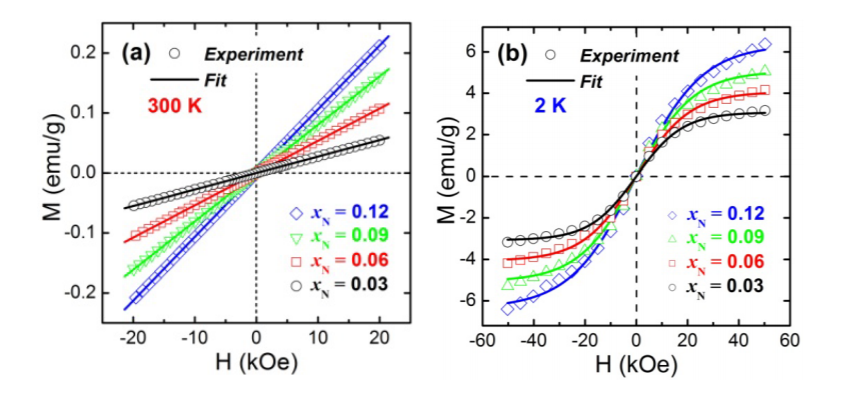
\includegraphics[width=0.99\linewidth]{souza}
	\caption{Magnetization vs. applied field in $Ti_{(1-x)}Co_{x}O_{2}$ nanoparticles \cite{de2013structural}}
	\label{fig:TEM_PT}
\end{figure}
\FloatBarrier

\section{Origin of ferromagnetism in DMS}

Despite extensive research have been performed on DMS over last few decades, the true origin of ferromagnetism remains still unclear. The principle concept of DMS is to induce ferromagnetism by adding magnetic dopants in a non-magnetic semiconductor material. But Sunderasan \textit{et al.} showed that ferromagnetism might be found in non-magnetic materials if their particle size is in nanoscale range \cite{sundaresan2006ferromagnetism}. In their research, they found that variation of annealing temperature of undoped non-magnetic oxides like ZnO, $In_{2}O_{3}$, Ce$O_2$ and $Al_{2}O_{3}$ is related to observed dilute ferromagnetism. In explanation they attributed this phenomena to be controlled by the concentration of oxygen vacancies on surface of the nanoparticles. According to Sunderasan \textit{et al.} the surface oxygen vacancies create localized electron spin moments which follow Ruderman-Kittel-Kasuya-Yosida (RKKY) interaction. The RKKY interaction is basically a long range exchange interaction between d or f orbital electrons and it decays in an algebraic manner with respect to the distance between spins. The theory of RKKY type exchange interaction was inspired from mean field Zener model which pioneered the theoretical proof of DMS properties in Mn doped II-VI and III-V semiconductors. \\

Zener model suggests that delocalized charge carriers enhances the ferromagnetic interaction of localized spins in metallic system. But the exchange interaction in DMS is different than the short range d-d exchange interaction in 3d metal. Applying the mean field theory to the Zener model, it's found that the ferromagnetism in DMS can be well described by the long range p-d exchange interaction between localized and delocalized spins. According to this theory, doped holes redistribute themselves by maintaining favorable delocalization length so that the energy of the system becomes less. The mean field Zener model established an exchange constant ($J_{p-d}$) which can be experimentally determined. This model not only predicted a number of DMS candidates including zinc blende and wurzite type wide band gap oxides and nitrides but also presented a mechanism to increase curie temperature in those materials. According to the suggestion, cure temperature can be raised by enhancing the hybridization energy which is proportional to $a^{-3}$ ($a$ is the lattice constant). 

\begin{figure}[!htb]
\centering
	\begin{subfigure}[h]{0.45\textwidth}
		\centering
		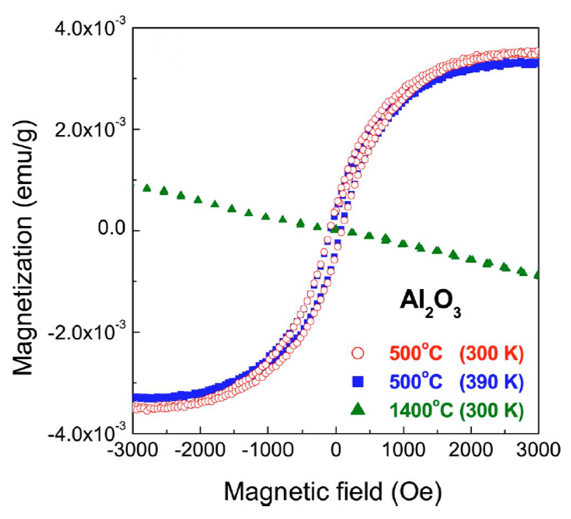
\includegraphics[width=\linewidth]{sunderasan_al2o3}
  		\caption{}
   		%\label{fig:sub-first}
	\end{subfigure}
	\begin{subfigure}[h]{0.46\textwidth}
		\centering
		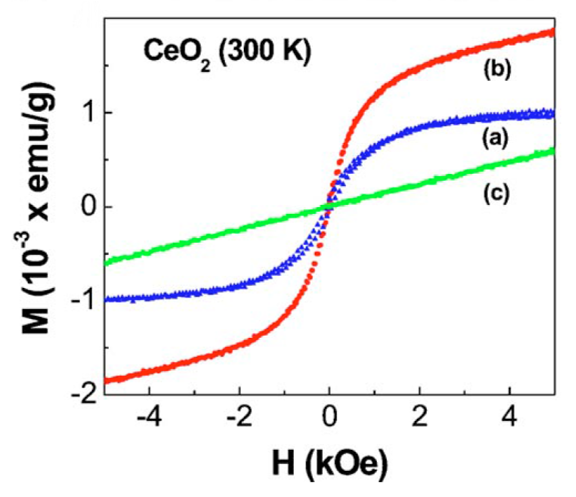
\includegraphics[width=\linewidth]{sunderasan_ceo2}
  		\caption{}
   		%\label{fig:sub-first}
	\end{subfigure}
	\begin{subfigure}[h]{0.45\textwidth}
		\centering
		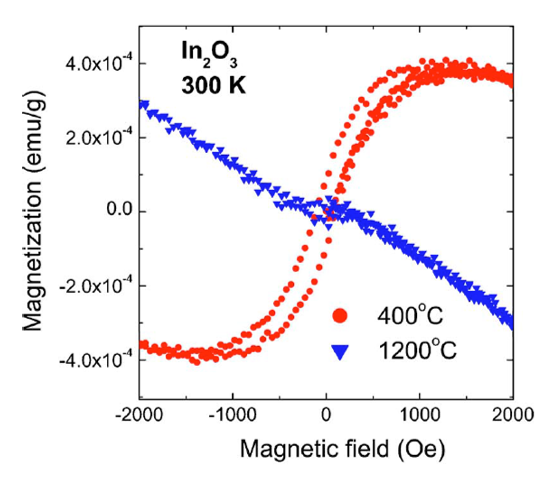
\includegraphics[width=\linewidth]{sunderasan_in2o3}
  		\caption{}
   		%\label{fig:sub-first}
	\end{subfigure}
	\begin{subfigure}[h]{0.47\textwidth}
  		\centering
  		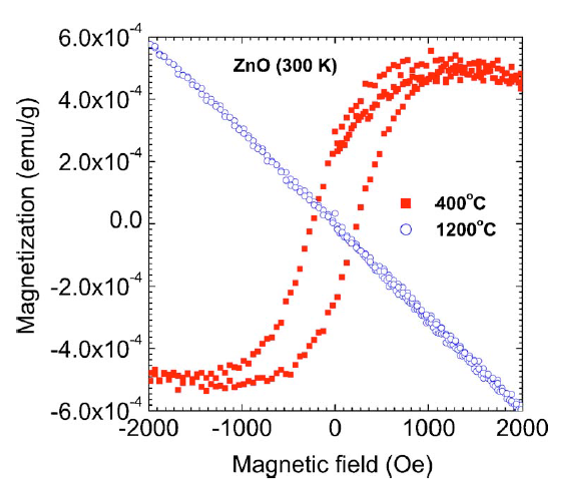
\includegraphics[width=\linewidth]{sunderasan_zno}
  		\caption{}
  		%\label{fig:sub-second}
	\end{subfigure}
\caption{Dilute ferromagnetism observed in undoped non-magnetic oxides due to oxygen vacancies \cite{sundaresan2006ferromagnetism}} 
\label{fig:fig}

\end{figure}
\FloatBarrier


\begin{figure}[!htb]
	\centering
	\includegraphics[width=0.8\linewidth]{rkky}
	\caption{RKKY type exchange interaction of frustrated spins in $CePO_{4}$ \cite{al2018effect}}
	\label{fig:TEM_PT}
\end{figure}
\FloatBarrier

The mean field Zener model predicted p-type DMS candidates where the hole induced bands will be just above the valence band. This theory was proved wrong when it was found that the predicted DMS candidates showed n-type semiconducting behavior. Actually Zener model considered d orbital electrons will not participate in charge transport and it was based on Mn induced band states. The case is different for other transition metal ions as Mn has a unique orbital levels which is not like the other transition metal ions. However, RKKY interaction resolved the issue which focused on charge carrier mediated interaction in the DMS. The concept of mean field Zener model and RKKY is almost same. RKKY explains the ferromagnetic-antiferromagnetic interaction when the concentration of holes is larger than that of spins which cannot be explained by Zener model. \\

In contrast to direct and indirect exchange interaction described by mean field Zener model and RKKY model, there are also some additional exchange interaction which have been found non-trivial to explain the ferromagnetism in DMS. Among them the concept of bound magnetic polaron is most relevant. When the delocalized spins act as a cluster and their behavior is controlled by the effective mass of the cluster. The polaronic interaction increases with decrease in temperature. The interaction between the localized polaron is antiferromagnetic. This model has become popular to explain the ferromagnetism observed in a low carrier density DMS. It is noteworthy to mention that none of these theories can alone truly describe the universal nature of the ferromagnetism in DMS. 

\section{Role of oxygen vacancy in oxide based DMS}

Oxide based DMS have showed high promises for room temperature intrinsic ferromagnetic behavior but the fundamental limitation is the true understanding of ferromagnetism in these materials. Oxygen vacancies play crucial role in determination of ferromagnetic interaction which have extensively studied by both computational and experimental approaches. In previous section, the research of Sunderasan \textit{et al.} clearly demonstrated the influence of oxygen vacancies on the observed ferromagnetism in undoped non-magnetic oxides. Oxygen vacancy induced band states strongly interact with delocalized electrons and are capable of nullifying the non-zero spin polarization at fermi level. Hence the role of oxygen vacancy has been deliberately studied since the discovery of intrinsic ferromagnetism in $Co:TiO_{2}$. \\

Bryan \textit{et al.} showed that the oxygen vacancies at grain boundaries are responsible for the high curie temperature ferromagnetism in Cr and Co doped $TiO_{2}$ nanomaterials \cite{bryan2005activation}. Chowdhury \textit{et al.} reported that Mn doping distorts the $TiO_{2}$ crystal structure generating oxygen vacancies at surface which reduce the mobility of charge carriers. They attributed the ferromagnetic interaction to be controlled by oxygen vacancies via forming bound magnetic polarons in the system \cite{choudhury2013oxygen}. Such kind of surface oxygen vacancy induced ferromagnetism has been reported for $TiO_{2}$, $SnO_{2}$, $TiO_{2}$ and $ZnO$ in many literatures \cite{santara2014oxygen, chen2010oxygen, chang2012oxygen, lee2002study, hong2005role, fernandes2009dilute}. 

\begin{figure}[!htb]
\centering
	\begin{subfigure}[h]{0.35\textwidth}
		\centering
		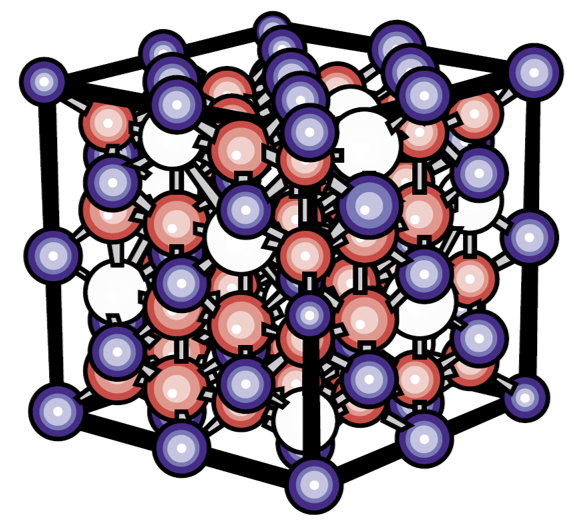
\includegraphics[width=\linewidth]{ceo2}
  		\caption{Stoichiometric Crystal Structure of $CeO_{2}$-$Ce_{2}O_{3}$. Blue, Red and White spheres indicate Cerium, Oxygen atoms $\&$ Oxygen vacancy}
   		%\label{fig:sub-first}
	\end{subfigure}
	\begin{subfigure}[h]{0.6\textwidth}
  		\centering
  		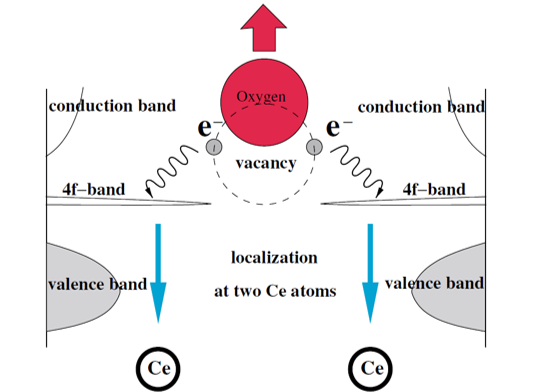
\includegraphics[width=\linewidth]{oxy_vacancy}
  		\caption{Oxygen vacancy leaves electron to its neighbor two $Ce^{4+}$ and they become $Ce^{4+}$}
  		%\label{fig:sub-second}
	\end{subfigure}
\caption{Role of oxygen vacancies in $CeO_{2}$ \cite{skorodumova2002quantum}} 
\label{fig:fig}

\end{figure}
\FloatBarrier


\section{Prospects of TiO$_{2}$ as DMS}

The groundbreaking discovery of Co:TiO$_{2}$ pioneered the quest for a DMS showing intrinsic semiconducting behavior at room temperature. Although, the prospects of DMS have been reported for other non-magnetic oxides like ZnO, $In_{2}O_{3}$ and Ce$O_2$, the superior stability of TiO$_{2}$ makes itself a unique candidate for DMS. For example, Ce$O_2$ has almost the similar lattice matching with Si but due to the unstability the DMS prospects in Ce$O_2$ are considered much volatile than the others. The exceptional capability of charge transfer between $Ce^{3+}$ and $Ce^{4+}$ enables Ce$O_2$ as an outstanding material for oxygen storage and catalyst like applications. But this unstability is a serious concern when it comes to any device application. From this perspective, TiO$_{2}$ outruns the other oxide DMS candidates. \\

$TiO_{2}$ has three stable polymorphs - anatase, rutile and brookite. Among them rutile is the most stable one in bulk and anastase is most stable in nanoscale range due to less surface energy \cite{satoh2013metastability}. Both anatase and rutile have tetragonal crystal structure while the titanium atom is surrounded by six oxygen atoms in an octahedral arrangement. During heat treatment, anatase undergoes a phase transition in the temperature range 600-700 $^{\circ}C$. Although, the bandgap of anatase (3.2 eV) is larger than rutile (3 eV), photoactivity of anatase is greater than the rutile due to anatase's electronic structure and surface morphology. \\

Transition and rare earth metal doped $TiO_{2}$ thin films and nanoparticles have been widely studied. Among them few literatures studied Sm doped $TiO_{2}$ nanoparticles and thin films. Xiao \textit{et al.} synthesized $Ti_{(1-x)}Sm_{x}O_{2}$ (0$\leq$x$\leq$0.015) via sol-gel autocombustion technique. In their research they investigated the photocatalytic properties of rutile-anatase heterostructure and did not carry out the magnetic characterization \cite{xiao2007sol}. 

\begin{figure}[!htb]
\centering
	\begin{subfigure}[h]{0.6\textwidth}
		\centering
		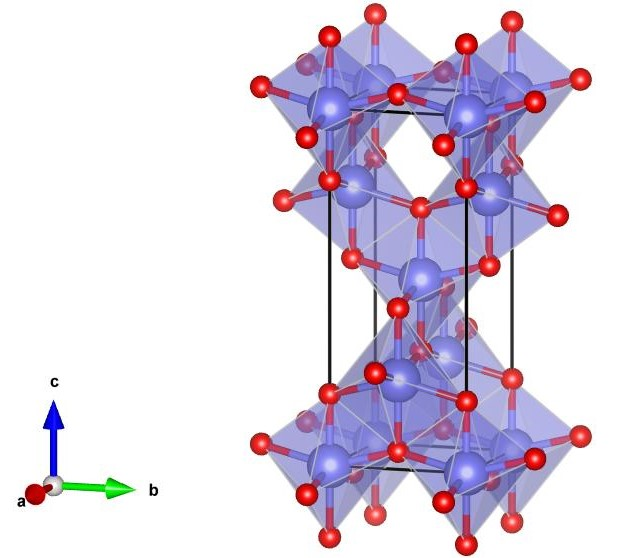
\includegraphics[width=\linewidth]{anatase}
  		\caption{Anatase ($a=b=3.78 \AA, c=9.51 \AA$)}
   		%\label{fig:sub-first}
	\end{subfigure}
	\begin{subfigure}[h]{0.6\textwidth}
		\centering
		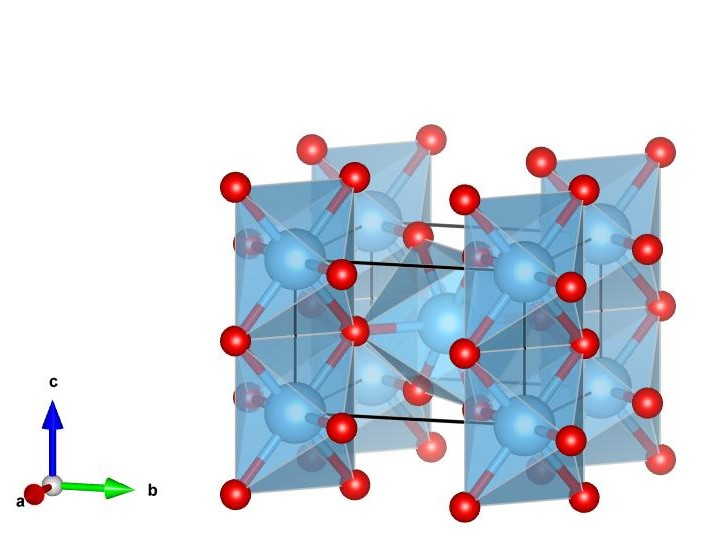
\includegraphics[width=\linewidth]{rutile}
  		\caption{Rutile ($a=b=4.59 \AA, c=2.95 \AA$)}
   		%\label{fig:sub-first}
	\end{subfigure}
	\begin{subfigure}[h]{0.6\textwidth}
  		\centering
  		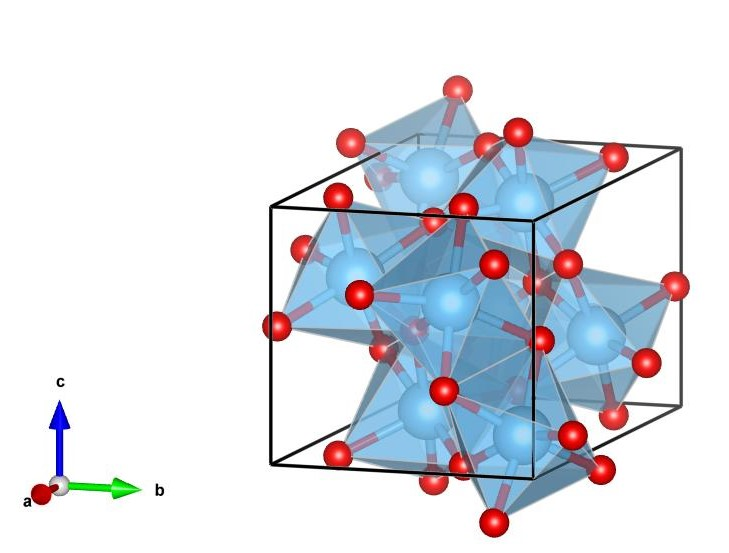
\includegraphics[width=\linewidth]{brookite}
  		\caption{Brookite ($a=5.45 \AA, b=9.18 \AA, c=5.14 \AA$)}
  		%\label{fig:sub-second}
	\end{subfigure}
\caption{Crystal Structure of three polymorphs of $TiO_{2}$ ($\alpha=\beta=\gamma=90^{\circ}$ for all polymorphs)} 
\label{fig:fig}

\end{figure}
\FloatBarrier

\begin{figure}[!htb]
	\centering
	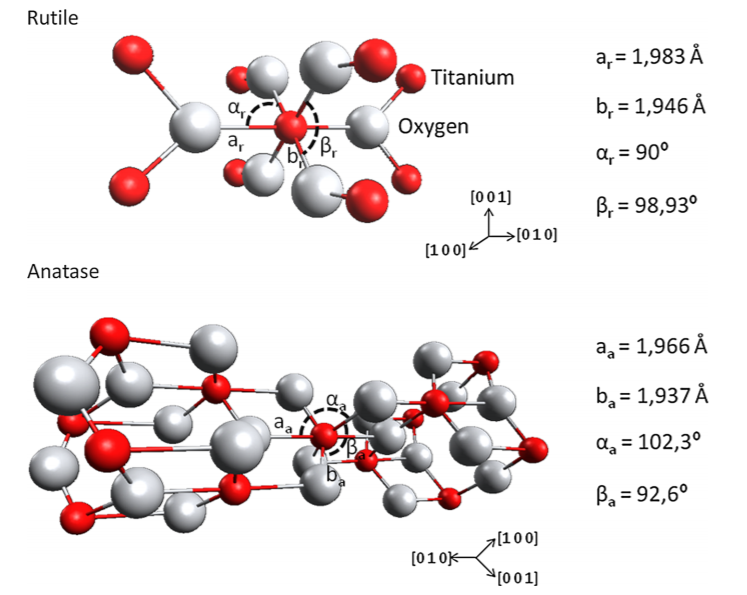
\includegraphics[width=0.6\linewidth]{bond_tio2}
	\caption{Difference in bond length and bond angles in rutile and anatase $TiO_{2}$}
	\label{fig:TEM_PT}
\end{figure}
\FloatBarrier

Cao \textit{et al.} synthesized $Ti_{(1-x)}Sm_{x}O_{2}$ (0$\leq$x$\leq$0.08) via sol-gel technique \cite{cao2013luminescence}. Above $550 ^{\circ}C$ anatase to rutile phase transition strated which became complete above $750 ^{\circ}C$. The authors have investigated the absorption spectra but they also did not characterizae the magnetic property of the samples. Shi \textit{et al.} also investigated the photocatalytic properties of $Ti_{0.99}Sm_{0.01}O_{2}$ nanoparticles and observed that Sm doping suppressed the particle size. The reduction in particle size was attributed to be beneficial in photocatalytic properties of the nanoparticles \cite{shi2008photocatalytic}. Hu \textit{et al.} studied luminiscence properties of Sm:Ti$O_2$ nanoparticles and reported highest luminiscenece for 0.75 mol$\%$ Sm:Ti$O_2$ nanoparticles \cite{hu2007photoluminescence}. Promising photoluminiscence and photocatalytic properties of Sm:Ti$O_2$ were also reported in some other literatures \cite{kiisk2005photoluminescence, park2011photoluminescence, dinkar2016sm, ma2010synthesis, xiang2017enhanced}. None of the above mentioned research work investigated the ferromagnetic behavior of the synthesized samples. Tseng \textit{et al.} synthesized rutile $Ti_{(1-x)}Sm_{x}O_{2}$ (0$\leq$x$\leq$0.02) by molten salt method and observed that dilute ferromagnetism of Sm doped Ti$O_2$ became weaker than the ferromagnetism of undoped Ti$O_2$ nanoparticles  \cite{tseng2016magnetic}. However, no detailed study on Sm:Ti$O_2$ has been reported so far to the best knowledge of the author of this thesis.  




\thispagestyle{fancy}


\end{document}







